%!TEX root = ../template.tex
%%%%%%%%%%%%%%%%%%%%%%%%%%%%%%%%%%%%%%%%%%%%%%%%%%%%%%%%%%%%%%%%%%%%
%% chapter4.tex
%% NOVA thesis document file
%%
%% Chapter with a short latex tutorial and examples
%%%%%%%%%%%%%%%%%%%%%%%%%%%%%%%%%%%%%%%%%%%%%%%%%%%%%%%%%%%%%%%%%%%%

\typeout{NT FILE chapter4.tex}%


\chapter{Case Study and Performance Analysis}
\label{cha:case_study}


% ===================================================================
%
% Section : Introduction
% ===================================================================

\section{Introduction}
\label{sec:case_study_intro}
isto pa \cite{tavaresgomes2026}


Having detailed the design and implementation of the automated code generation tool in Chapter \ref{cha:chap_3}, this chapter now seeks to validate its practical utility and analyze its output in a real-world scenario. Although the previous chapter verified the tool's functionality, this chapter demonstrates its application within the intended model-driven development workflow, from a high-level system specification to a deployed multi-controller system [cite: 1, 2, 3].

To achieve this, a case study is presented centered on a distributed controller for a three-conveyor automation system [cite: 3]. This application was chosen because it represents a common class of problems in industrial automation, involving multiple coordinated subsystems. The implementation of this case study serves two primary objectives, directly adapted from the research goals presented in [cite: 3]:

\begin{enumerate}
    \item \textbf{To validate the end-to-end development workflow:} This involves demonstrating how the IOPT-Tools framework and the newly developed API are jointly employed to support low-code development of a distributed system. The process begins with a global IOPT model, proceeds through model decomposition, and culminates in the automatic generation and integration of both the controller logic and heterogeneous communication modules [cite: 3].
    
    \item \textbf{To conduct a quantitative performance analysis:} By implementing intercontroller communication using three distinct protocols, I2C, UART, and TCP/MQTT. This chapter provides an empirical comparison of their respective resource overheads. ]The analysis focuses specifically on the memory footprint, offering valuable insight into the trade-offs associated with each protocol in a resource-constrained embedded environment [cite: 3].
\end{enumerate}

This chapter begins by describing the conveyor system use case and its corresponding IOPT model. Then it details the implementation process, showing how the automated tool was used to generate the necessary communication code. Subsequently, the results of the performance analysis are presented and discussed. The chapter concludes with a summary of the key findings of the case study.


% = =================================================================
% Use Case Description
% ===================================================================
\section{Use Case Description: The Three-Conveyor System}
\label{sec:use_case_description}

To demonstrate the practical application of the development workflow, a case study from the industrial automation domain was selected. The system under consideration is a controller for a three-conveyor belt set-up, designed to transport items sequentially from an entrance point to an exit point.

As illustrated in Figure \ref{fig:conveyor_layout}, the physical system consists of three different conveyors. Each conveyor is equipped with two sensors to detect the presence of an item: one at its entrance (\texttt{in1}, \texttt{in2}, \texttt{in3}) and one at its exit (\texttt{out1}, \texttt{out2}, \texttt{out3}). An additional sensor (\texttt{in4}) detects when an item is removed from the end of the final conveyor. Control actions involve activating the motor for each of the three conveyors (\texttt{move1}, \texttt{move2}, \texttt{move3}). The objective of the controller is to ensure that the items move smoothly throughout the system, and each conveyor is activated only when an item is ready to be transferred and the subsequent conveyor is clear.

\begin{figure}[htb]
    \centering
    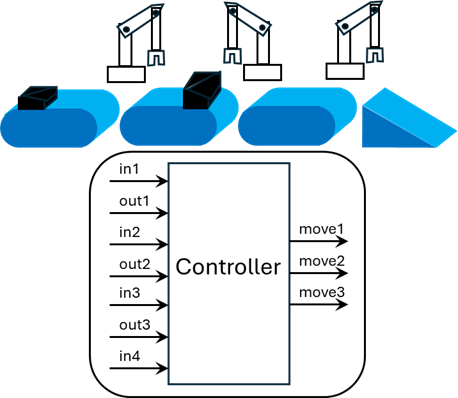
\includegraphics[width=0.6\columnwidth]{Chapters/Figures/layout.png}
    \caption{Layout of the three-conveyor system, showing the placement of sensors and the direction of item flow.}
    \label{fig:conveyor_layout}
\end{figure}

The complete centralized behavior of the controller is formally specified using the single global IOPT Petri net model shown in Figure \ref{fig:global_model}. For clarity and brevity in this case study, the model assumes that each conveyor has a capacity of a single item. This global model represents the entire system logic before any consideration of a distributed implementation.

\begin{figure}[htb]
    \centering
    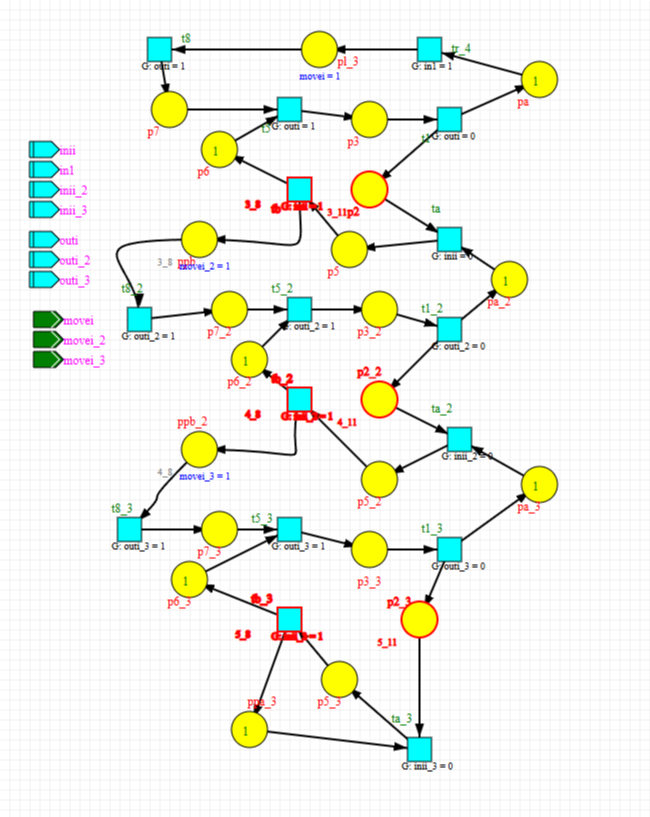
\includegraphics[width=0.95\columnwidth]{Chapters/Figures/modeloglobalcomcuttingset.png}
    \caption{The global IOPT Petri net model specifying the centralized controller for the entire conveyor system. The nodes highlighted in red represent the chosen cutting set for decomposition.}
    \label{fig:global_model}
\end{figure}

For deployment onto a set of distributed hardware controllers, the global model was decomposed using the net splitting operation available in IOPT-Tools. A cutting set, consisting of three places and three transitions (highlighted in red in Figure \ref{fig:global_model}), was selected to partition the model along the physical boundaries of the three conveyors. The result of this operation is shown in Figure \ref{fig:decomposed_model}. The original centralized model is transformed into a set of four interconnected, concurrent sub-models, each responsible for a portion of the system (Entrance, Conveyor Two, Conveyor Three, and Exit). The connections between these submodels represent the abstract communication channels that must be implemented to ensure the correct synchronized behavior of the distributed system.

\begin{figure*}[htb]
    \centering
    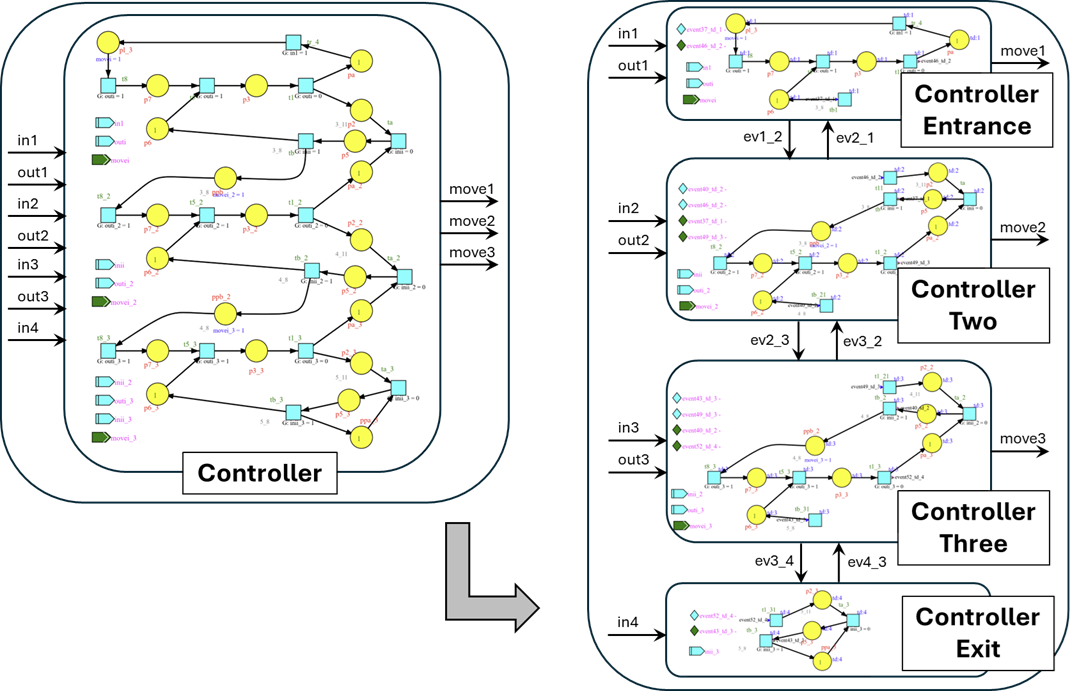
\includegraphics[width=0.9\textwidth]{Chapters/Figures/controller_decomposition.png}
    \caption{The transformation from the centralized controller model (left) to a set of concurrent, networked sub-models (right) resulting from the net splitting operation.}
    \label{fig:decomposed_model}
\end{figure*}


% ===================================================================
% Section 4.3: Implementation via Automated Code Generation
% ===================================================================
\section{Implementation via Automated Code Generation}
\label{sec:use_case_implementation}

With the global IOPT model decomposed into a set of concurrent sub-models (as shown in Figure \ref{fig:decomposed_model}), the next step in the development workflow is to implement the abstract communication channels between them. This task was accomplished using the automated code generation API detailed in Chapter 3.

The target deployment architecture for this case study, shown in Figure \ref{fig:deployment_layout}, employs a heterogeneous mix of three different communication protocols to connect the four controller modules. The following subsections detail how the specific code for each communication link was generated using the API.

\begin{figure*}[htb]
    \centering
    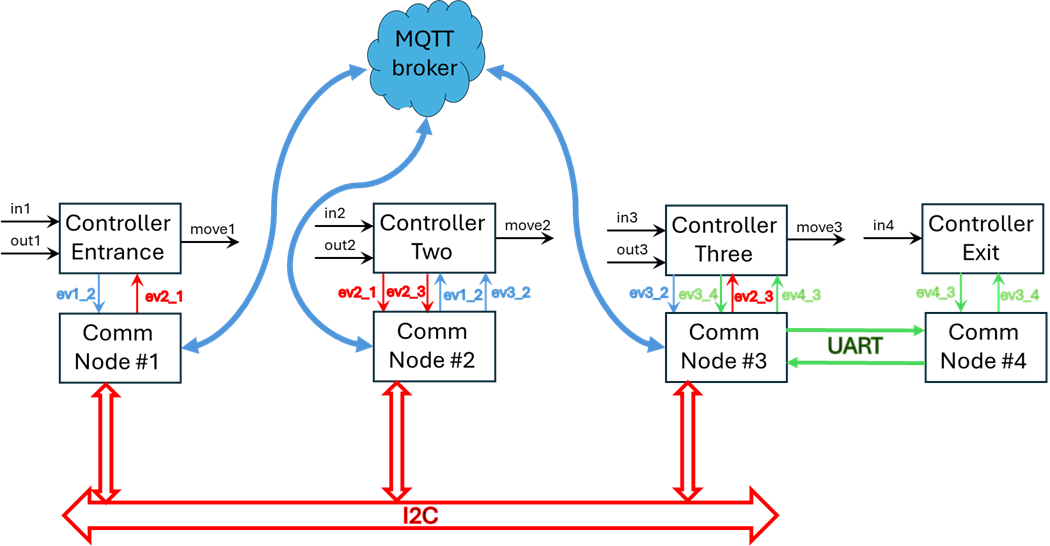
\includegraphics[width=1\textwidth]{Chapters/Figures/prototypelayout.png}
    \caption{The heterogeneous deployment architecture for the distributed conveyor system controller, utilizing I²C, UART, and MQTT over TCP/IP for inter-controller communication and synchronization.}
    \label{fig:deployment_layout}
\end{figure*}

\subsection{I²C Bus Implementation}
As depicted in the deployment architecture, \textit{Controller Two} acts as the master on a local I²C bus, coordinating with \textit{Controller Entrance} and \textit{Controller Three}, which act as slaves. To generate the necessary master and slave code for an event representing a piece transfer, an API call similar to the following was used:

\begin{verbatim}
?protocol=i2c&projectName=ControllerTwo&eventName=TransferReady&
slaveAddress=8&slaveMessage=R
\end{verbatim}

% Inside Section 4.3.1

A validation of this bus's dynamic behavior, showing the sequence of events between the master and slaves, is presented and analyzed in detail in Section 4.4.4(mudar) via a simulator-captured timing diagram.


\subsection{UART Point-to-Point Link}
A direct, asynchronous serial link between \textit{Controller Three} and \textit{Controller Exit} was required to signal the final transfer of a piece. The code for this UART-based communication was generated with the following API call:

\begin{verbatim}
?protocol=uart&projectName=ControllerThree&eventName=PieceExiting&
baudRate=115200
\end{verbatim}

\subsection{MQTT Network Communication}
To handle higher-level, asynchronous status updates between the main controllers, the MQTT protocol was employed over a Wi-Fi network. For example, to allow \textit{Controller Entrance} to publish a "Part Arrived" event to a central topic that \textit{Controller Two} subscribes to, the following API call was made:

\begin{verbatim}
?protocol=tcp&projectName=ControllerEntrance&eventName=PartArrived&
topic=conveyor/status
\end{verbatim}

\subsection{Code Integration}
For each controller, the specific communication modules generated by the API calls were integrated with the logic code of the baseline controller produced by the standard IOPT-Tools generator. The entire process of specifying, generating, and integrating the code for all three heterogeneous communication links was completed in a fraction of the time required for manual implementation. This successfully demonstrates the tool's primary objective: to accelerate the development of distributed control systems and reduce the potential for implementation errors by automating the creation of communication infrastructure.



% ===================================================================
% Section 4.4: Performance Analysis and Results
% ===================================================================
\section{Performance Analysis and Results}
\label{sec:performance_analysis}

After successfully implementing the distributed controller for the conveyor system, a performance analysis was performed to quantify the resource overhead associated with the different communication protocols generated by the tool. Although multiple performance metrics such as latency and CPU usage could be considered, this analysis focuses on the **memory footprint**, as it is often the most critical constraint in embedded systems development.

\subsection{Methodology}
\label{subsec:analysis_methodology}

The memory footprint of each of the four controller modules (Entrance, Two, Three and Exit) was measured to determine the overhead of its communication stack. The process was as follows.
\begin{enumerate}
    \item \textbf{Baseline Measurement:} For each controller, the code containing only the Petri net execution logic (generated by the standard IOPT-Tools) was compiled for the ESP32 target. The static program storage space (Flash memory) reported by the compiler was recorded as the baseline.
    \item \textbf{Measurement with Communication:} The API-generated communication code, corresponding to the heterogeneous architecture shown in Figure \ref{fig:deployment_layout}, was integrated with the baseline logic for each controller. The project was then recompiled and the new total program size was recorded.
    \item \textbf{Overhead Calculation:} The communication overhead was calculated as the difference in memory footprint between the baseline measurement and the measurement with the integrated communication code.
\end{enumerate}

\subsection{Results}
\label{subsec:analysis_results}

The results of the memory footprint analysis are summarized in Table \ref{tab:memory_footprint}. The data reveals a significant variation in overhead that is strongly correlated with the complexity of the communication protocols implemented on each controller module.

\begin{table}[htb]
\centering
\small % Reduce the font size for the table
\caption{Memory Analysis of Controller Implementations.}
\label{tab:memory_footprint}
\sisetup{group-separator={,}}
% Using abbreviated headers to save space
\begin{tabular}{l S[table-format=6.0] S[table-format=6.0] S[table-format=5.0] S[table-format=1.2]}
\toprule
\textbf{Controller} & {\textbf{Baseline}} & {\textbf{W/ Comm.}} & {\textbf{Overhead}} & {\textbf{Overhead}} \\
& {\textbf{(B)}} & {\textbf{(B)}} & {\textbf{(B)}} & {\textbf{(\%)}} \\
\midrule
Entrance & 927970 & 954178 & 26208 & 2.82 \\
Two & 928578 & 955894 & 27316 & 2.94 \\
Three & 928642 & 957014 & 28372 & 3.06 \\
Exit & 927058 & 928478 & 1420  & 0.15 \\
\bottomrule
\end{tabular}
\end{table}

\subsection{Discussion of Results}
\label{subsec:analysis_discussion}

The data presented in Table \ref{tab:memory_footprint} clearly illustrate the critical trade-off between functional flexibility and resource consumption when selecting a communication protocol.

The \textbf{Entrance Controller} and \textbf{Controller Two}, both of which implement a full TCP/IP stack for MQTT messaging along with I2C, exhibit the most substantial overheads at approximately 26.2 and 27.3 kB, respectively. This confirms that network-level protocols are the main contributors to the memory footprint. The complexity of the TCP/IP stack, which requires significant buffer space and state management for reliable communication, combined with the MQTT client library, accounts for the vast majority of this resource cost.

This is further corroborated by the data from the \textbf{Exit Controller}. This module, which implements \textit{only} the UART protocol for simple point-to-point asynchronous communication, shows a remarkably low overhead of just 1,420 bytes (a mere 0.15\% increase). This stark contrast highlights the lightweight nature of hardware-level serial protocols compared to their network-level counterparts, as the former can be implemented with minimal software abstraction.

These findings have significant implications for the design of distributed embedded systems. The model-driven development approach, augmented by the tool presented in this thesis, allows a designer to make informed decisions during the system partitioning phase. By analyzing the communication requirements of each sub-model, complex and memory-intensive protocols like TCP/MQTT can be selectively deployed only on controllers that require network connectivity. Simpler nodes can be implemented with lightweight protocols like UART or I2C, thus optimizing the overall system's resource usage and ensuring that hardware constraints are met.

% ===================================================================
% Section 4.5: Chapter Summary
% ===================================================================
\section{Chapter Summary}
\label{sec:case_study_summary}

This chapter successfully demonstrated the practical application and value of the automated code generation tool through a detailed case study of a three-conveyor distributed control system. The work presented herein validated the entire model-driven development workflow, beginning with a high-level IOPT Petri net model and culminating in a functional, multi-controller hardware implementation. The tool was shown to seamlessly integrate into this workflow, allowing the rapid and reliable implementation of a complex and heterogeneous communication architecture that involves the I2C, UART and TCP / MQTT protocols.

Furthermore, the performance analysis provided critical, quantitative insights into the resource consumption of these protocols. The results empirically confirmed the significant memory overhead of network-level protocols like TCP/MQTT when compared to the lightweight nature of hardware-level protocols such as UART. Ultimately, this case study validates the central proposition of this thesis: that automated generation of communication modules not only accelerates development, but also empowers designers to make informed, data-driven decisions when balancing functional requirements against the hardware constraints of embedded systems.